\documentclass[UTF8]{ctexart}
\usepackage{geometry}
\usepackage{mathrsfs}
\usepackage{graphicx}
\usepackage{multirow}
\usepackage{amsmath}
\usepackage{amssymb}
\usepackage{array}
\usepackage{subfigure}
\usepackage{algorithm2e}
\usepackage{setspace}
\usepackage{diagbox}
\usepackage{bmpsize}
\usepackage{listings}
\geometry{a4paper,scale=0.75}
\newcommand{\xiaosi}{\fontsize{11.6pt}{\baselineskip}\selectfont}
\newcommand{\sihao}{\fontsize{12.1pt}{\baselineskip}\selectfont}
\newcommand{\upcite}[1]{\textsuperscript{\textsuperscript{\cite{#1}}}}
\renewcommand{\baselinestretch}{1.3}

%opening
\title{数字图像处理图像配准作业}
\author{赵子瑞 \\ 自动化钱61班}
\date{2019年3月5日}

\usepackage{xcolor}
\lstset{
	language = Python,
	basicstyle=\small,
    numbers=left, 
    numberstyle= \tiny, 
    keywordstyle= \color{ blue!70},
    commentstyle= \color{red!50!green!50!blue!50}, 
    frame=shadowbox, % 阴影效果
    rulesepcolor= \color{ red!20!green!20!blue!20} ,
    xleftmargin=2em,xrightmargin=2em, aboveskip=1em,
	framexleftmargin=1em,
	numbersep = 5pt,
	extendedchars=false
} 
\begin{document}

\maketitle

\newenvironment{cnabandkey}[2][\sihao 摘要] % 定义中文摘要和关键词环境
{\newcommand{\ckeywords}{#2} %
	\begin{center} \bfseries #1 \end{center} %
	\begin{quotation}
	}{\paragraph{\sihao 关键词:} \textrm{\ckeywords} %
	\end{quotation}
}

\newenvironment{enabandkey}[2][\sihao Abstract] % 定义英文摘要和关键词环境
{\newcommand{\ekeywords}{#2} %
	\begin{center} \bfseries #1 \end{center} %
	\begin{quotation}
	}{\paragraph{\sihao Keywords:} \textrm{\ekeywords} %
	\end{quotation}
}

	\begin{cnabandkey}{图像配准\, 图像处理\, 仿射变换\, 矩阵计算}
        \xiaosi
        \hspace{0.25em}本文是数字图像与视频处理的第二次作业,通过理论学习和代码实践,完成了以下任务:
        
		通过手动标点,得到图像中7个位置的坐标,进行输出并保存,计算仿射变换矩阵,通过仿射变换矩阵计算得到变换后的图像,输出图像。
		
		本次实验较为简单,建立在第一次实验的基础之上,提高了动手能力和对图像处理的理论理解。
		
	\end{cnabandkey}
	
	\clearpage



\xiaosi
\section{项目任务}

要求根据已给的两幅图像,在各幅图像中随机找出7个点,计算出两幅图像之间的转换矩阵H,并且输出转换之后的图像。
注:已给图像分别为$Image A$和$Image B$。

\section{手动标点}

本次实验中标定的点如图\ref{interest_point_selection}所示

\begin{figure}[h!]
	\centering
	\subfigure[原图像标定点选择]{
		\label{image_a} %%first figure label
		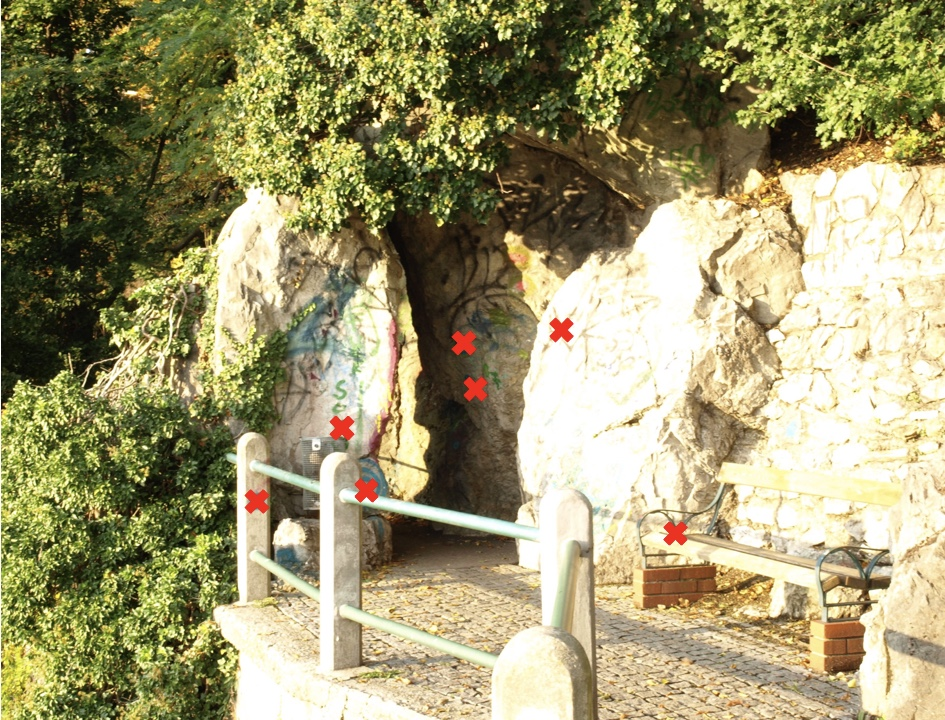
\includegraphics[width = 0.5\textwidth]{imgasele.jpg}}
	\hspace{0.1in} \subfigure[变换后图像选择]{
		\label{image_b} %%second figure label
		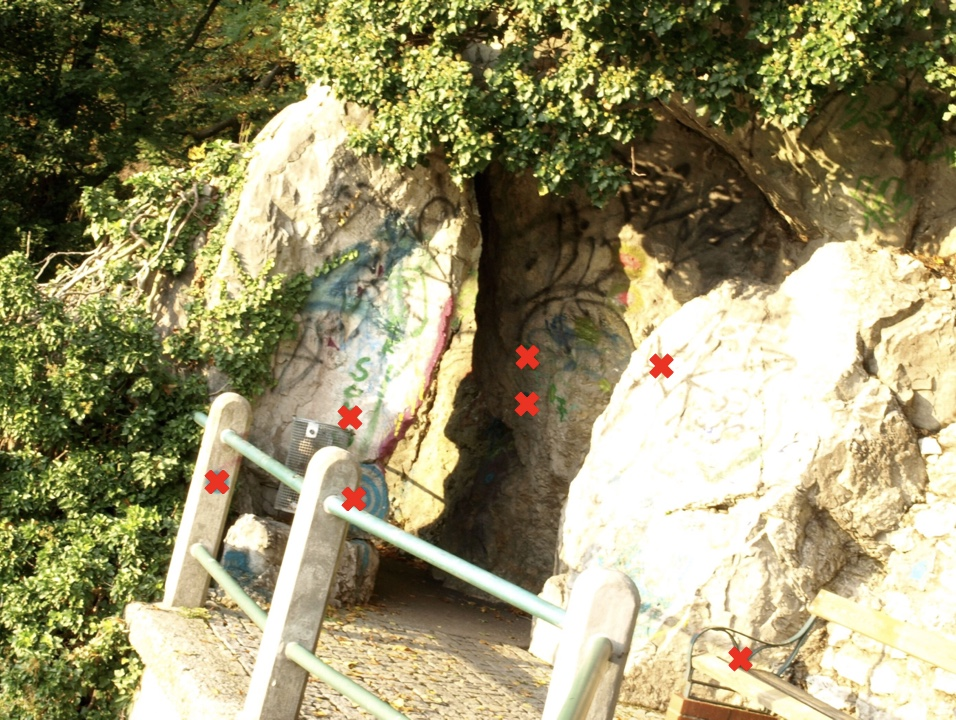
\includegraphics[width = 0.5\textwidth]{imgbsele.jpg}}	
	\caption{标定点选择} 
	\label{interest_point_selection} %%label for entire figure
\end{figure}

\section{输出两幅图中对应点的坐标}

得到的坐标输出如下。

Image A 的特征点如下。
\[ \begin{array}{cc}
	\left(977.693542 , 1919.11292\right) \\
	\left(1286.59680 , 1624.91931\right) \\
	\left(1374.85486 , 1867.62903\right) \\
	\left(1749.95166 , 1316.01611\right) \\
	\left(1786.72583 , 1448.40320\right) \\
	\left(2139.75806 . 1249.82263\right) \\
	\left(2581.04834 , 2022.08069\right) 
\end{array} \]

Image B选取的特征点坐标如下。
\[ \begin{array}{cc}
	\left(639.600830, 1397.73987\right) \\
	\left(1015.80042, 1201.21777\right) \\
	\left(1032.64514, 1453.88916\right) \\
	\left(1537.98792, 1010.31049\right) \\
	\left(1537.98792, 1161.91333\right) \\
	\left(1931.03223, 1066.45972\right) \\
	\left(2150.01416, 1925.54236\right) 
\end{array} \]

\section{计算转换矩阵}

转换矩阵的计算可以由公式\ref{Transform_Matrix}得到:
\begin{equation}
	\label{Transform_Matrix}
	H = Q \cdot P^T \cdot (P \cdot P^T )^{-1}
\end{equation},
其中,$P$为原图像的特征点组成的矩阵,$Q$为变换后对应的特征点组成的矩阵,$H$为变换矩阵。

经过计算,变换矩阵为:

\[\left( \begin{array}{ccc}
	0.958704864 & -0.263552481 & 208.122426  \\
	0.267151126 & 0.967908948 & -720.247315 \\
	0 & 0 & 1 
	\end{array} \right)\]

\section{输出在转换后的图像}

变换后的图像如图\ref{after_transform}所示。

\begin{figure}[h!]
	\centering
	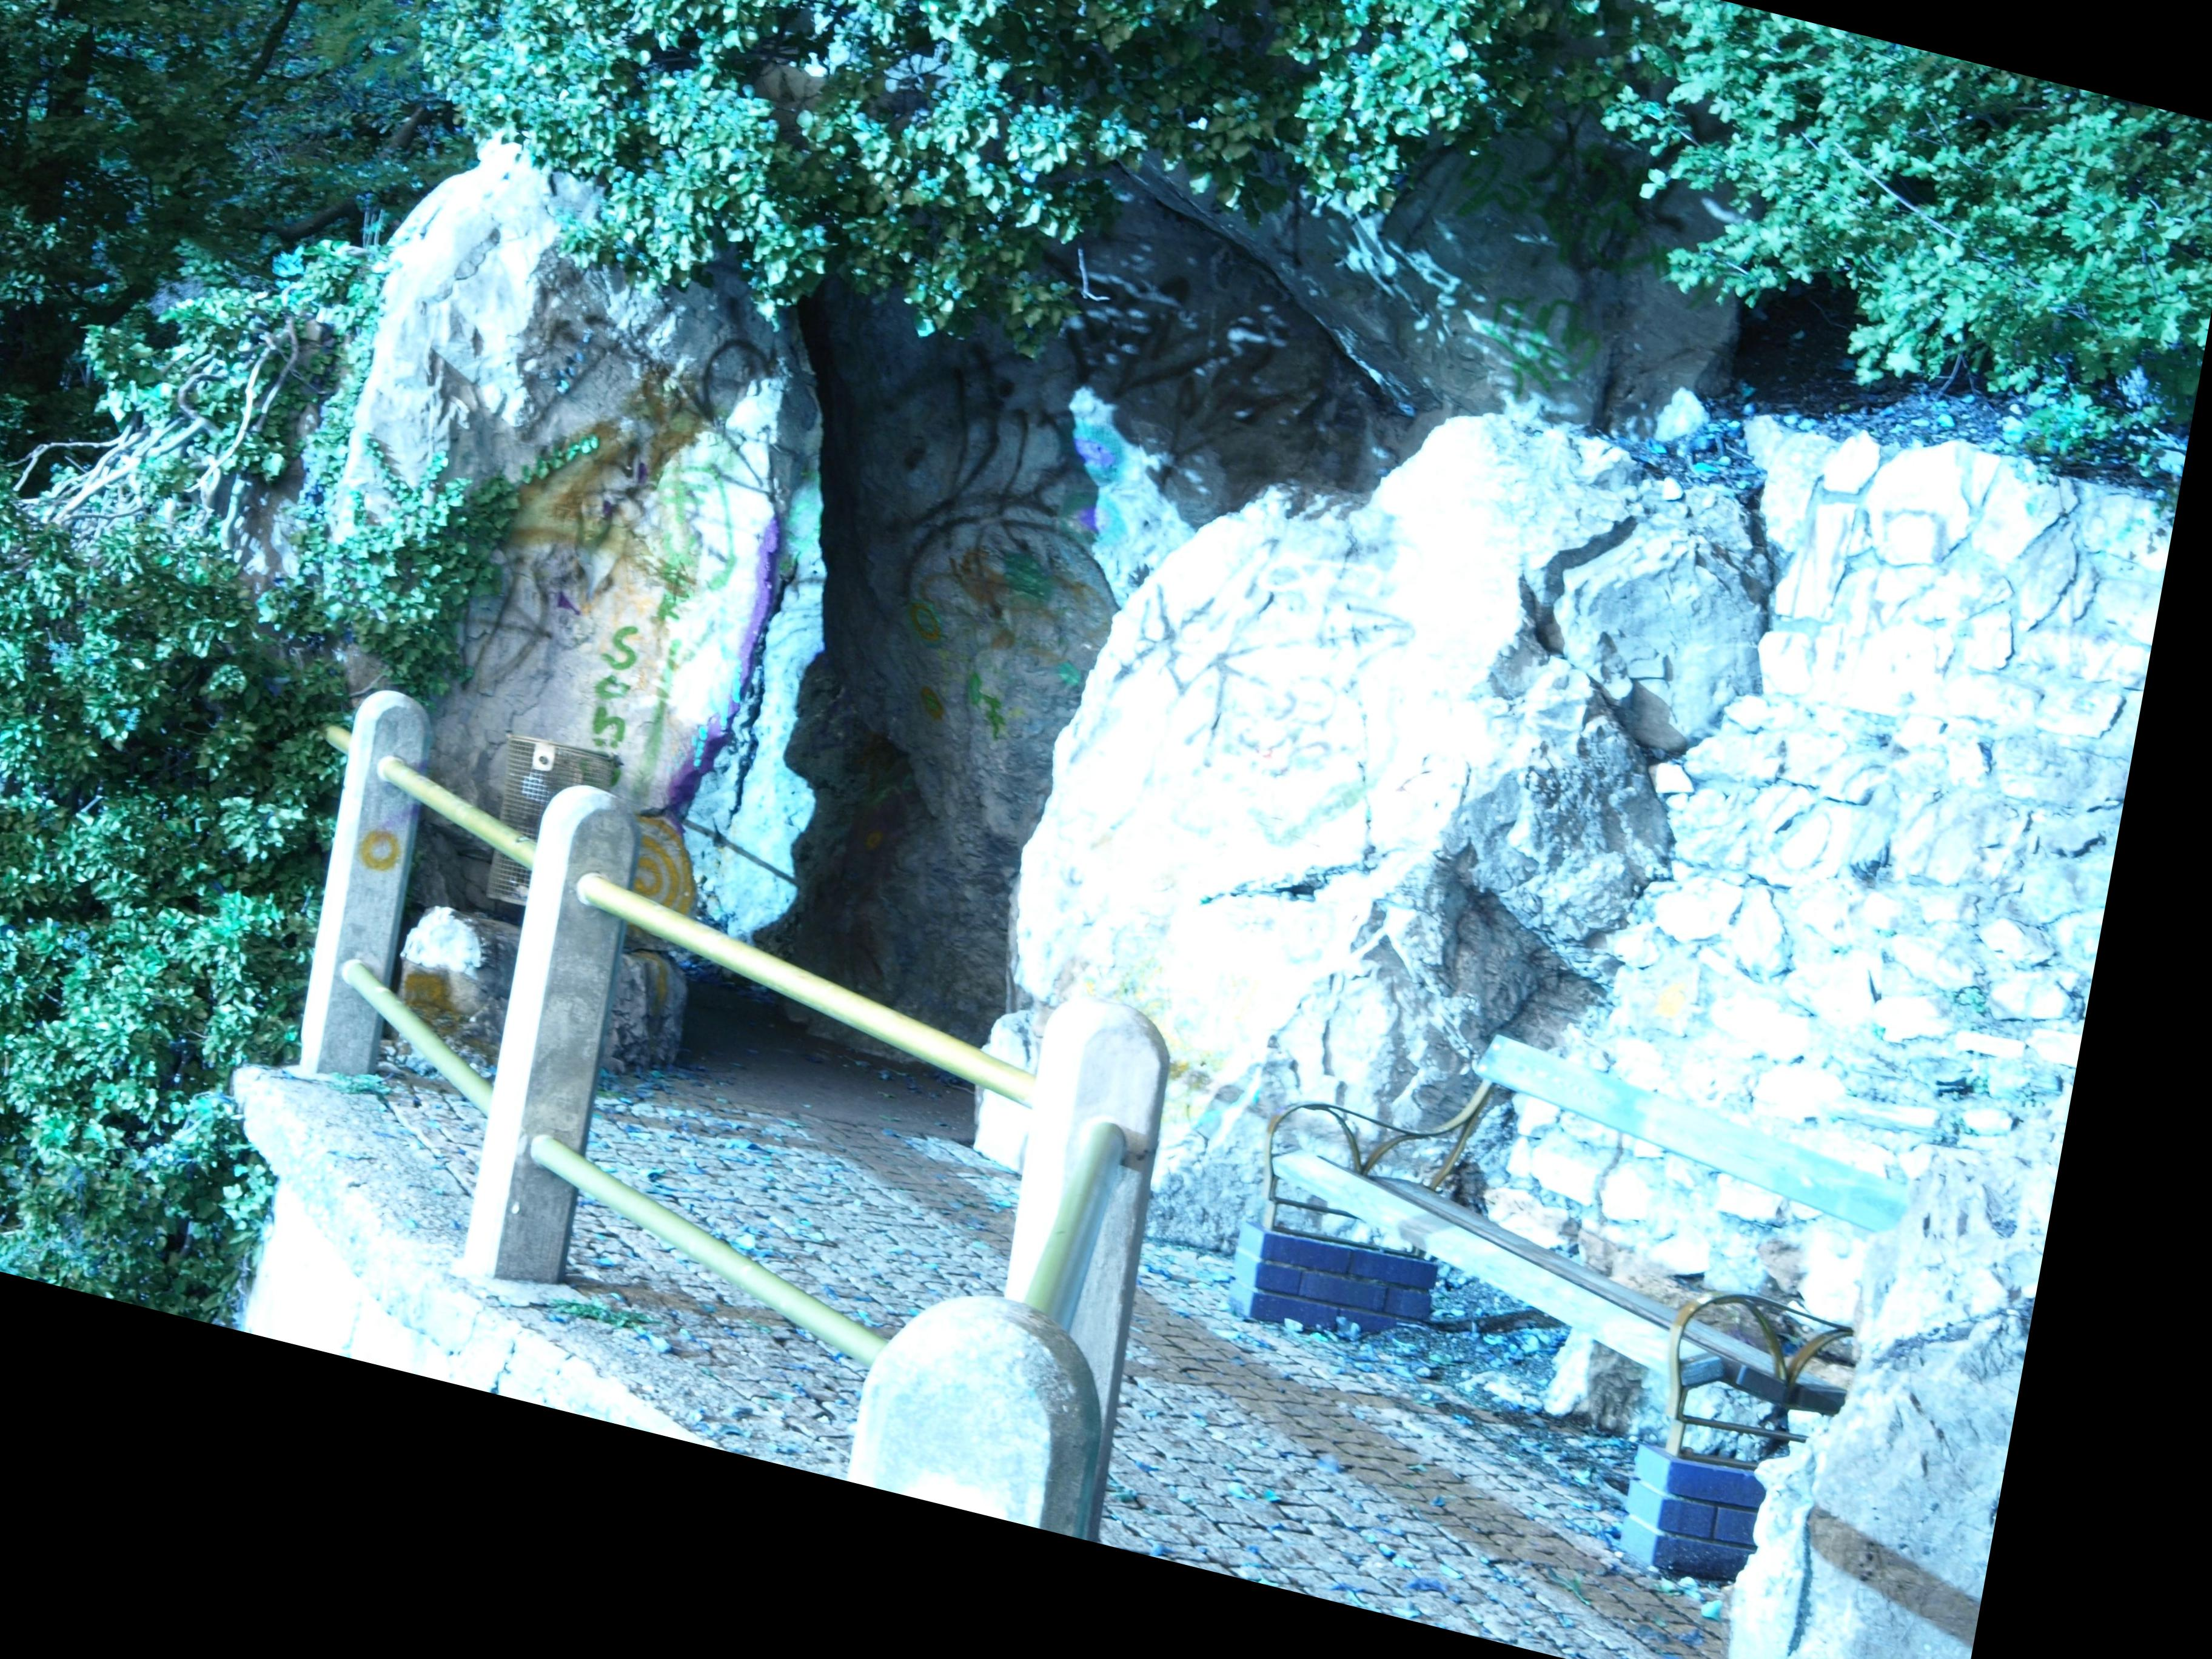
\includegraphics[width=0.65\linewidth]{test.jpg}
	\caption{变换后的图像}
	\label{after_transform}
\end{figure}

\section{代码示例}

\begin{lstlisting}
import cv2
import matplotlib.pyplot as plt
import base64
import struct
import numpy as np
from scipy import interpolate
from pylab import *
from PIL import Image

class basic_cv_tool:

	def __init__(self, ImageName):
		self.ImageName = ImageName

	def ImageRead(self, ImageName):
		img = cv2.imread(ImageName)
		return img
	
	def interest_point_choosing(self, ImageName):
		img = array(Image.open(ImageName))
		imshow(img)
		fea_point = ginput(7)
		fea_point = np.float32(fea_point)
		fea_point = np.column_stack((fea_point, \ 
		array([1,1,1,1,1,1,1])))
		return fea_point
	
	def Getting_H_Matrix(self, img_points_1, img_points_2):
		H_matrix = ((img_points_2.transpose()) \ 
		.dot(img_points_1)).dot(np.linalg.inv( \ 
		(img_points_1.transpose()).dot(img_points_1)))
		
		print(H_matrix)
		return H_matrix[:2]

if __name__ == '__main__':
	image_1_name = '../../homework2/Image A.jpg'
	image_2_name = '../../homework2/Image B.jpg'

	tool = basic_cv_tool(image_1_name)
	image = tool.ImageRead(image_1_name)
	print(image.shape)
	img1 = tool.interest_point_choosing(image_1_name)
	print("interest_point of image A is",img1)
	img2 = tool.interest_point_choosing(image_2_name)
	print("interest_point of image B is",img2)
	M = tool.Getting_H_Matrix(img1, img2)
	img = cv2.warpAffine(image, M, (image.shape[1], image.shape[0]))
	print(img.shape)
	cv2.imwrite('test.jpg', img)

\end{lstlisting}

\section{心得体会}

本次作业,通过实践,我深入了解了图像配准的相关基础知识,同时也提高了动手能力,加深了我对仿射变换的理解和掌握程度,也让我拥有了解决实际问题的基本功。同时,代码能力也得到了有效锻炼,
我的python能力得到了有效锻炼,同时也学习了opencv的很多基本功能。我自行组织的$cv toolbox$在我的$github$上维护,欢迎访问 \newline $https://github.com/1989Ryan/Digital-Image-Processing-Project$进行了解.


\end{document}